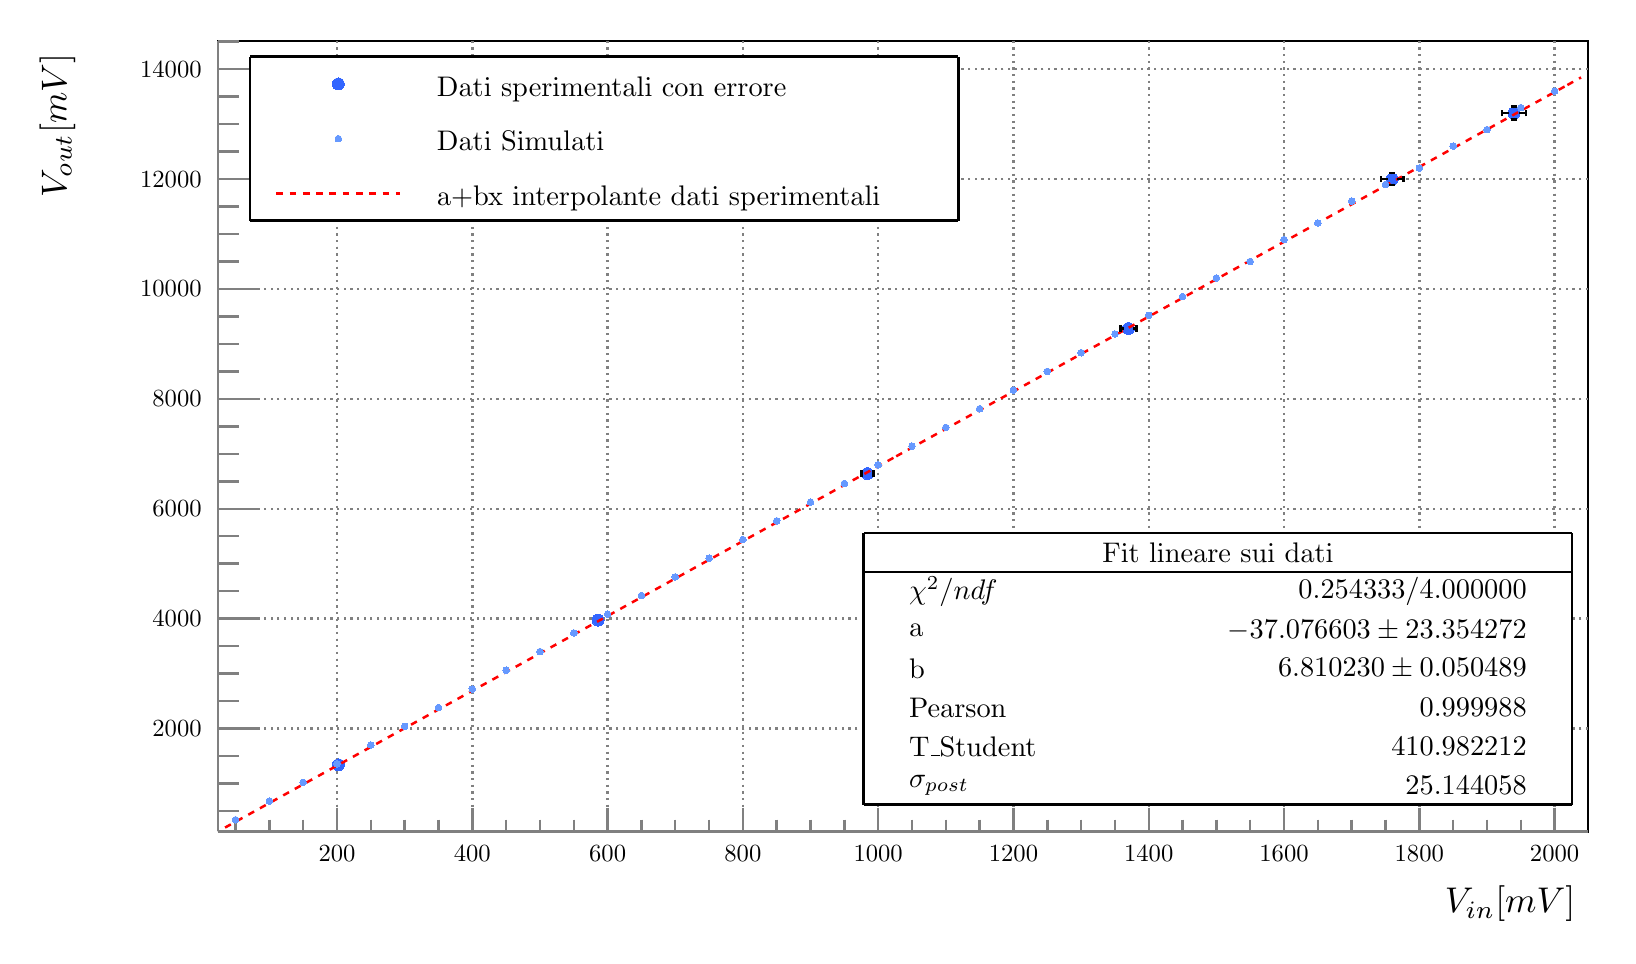
\begin{tikzpicture}
\pgfdeclareplotmark{cross} {
\pgfpathmoveto{\pgfpoint{-0.3\pgfplotmarksize}{\pgfplotmarksize}}
\pgfpathlineto{\pgfpoint{+0.3\pgfplotmarksize}{\pgfplotmarksize}}
\pgfpathlineto{\pgfpoint{+0.3\pgfplotmarksize}{0.3\pgfplotmarksize}}
\pgfpathlineto{\pgfpoint{+1\pgfplotmarksize}{0.3\pgfplotmarksize}}
\pgfpathlineto{\pgfpoint{+1\pgfplotmarksize}{-0.3\pgfplotmarksize}}
\pgfpathlineto{\pgfpoint{+0.3\pgfplotmarksize}{-0.3\pgfplotmarksize}}
\pgfpathlineto{\pgfpoint{+0.3\pgfplotmarksize}{-1.\pgfplotmarksize}}
\pgfpathlineto{\pgfpoint{-0.3\pgfplotmarksize}{-1.\pgfplotmarksize}}
\pgfpathlineto{\pgfpoint{-0.3\pgfplotmarksize}{-0.3\pgfplotmarksize}}
\pgfpathlineto{\pgfpoint{-1.\pgfplotmarksize}{-0.3\pgfplotmarksize}}
\pgfpathlineto{\pgfpoint{-1.\pgfplotmarksize}{0.3\pgfplotmarksize}}
\pgfpathlineto{\pgfpoint{-0.3\pgfplotmarksize}{0.3\pgfplotmarksize}}
\pgfpathclose
\pgfusepathqstroke
}
\pgfdeclareplotmark{cross*} {
\pgfpathmoveto{\pgfpoint{-0.3\pgfplotmarksize}{\pgfplotmarksize}}
\pgfpathlineto{\pgfpoint{+0.3\pgfplotmarksize}{\pgfplotmarksize}}
\pgfpathlineto{\pgfpoint{+0.3\pgfplotmarksize}{0.3\pgfplotmarksize}}
\pgfpathlineto{\pgfpoint{+1\pgfplotmarksize}{0.3\pgfplotmarksize}}
\pgfpathlineto{\pgfpoint{+1\pgfplotmarksize}{-0.3\pgfplotmarksize}}
\pgfpathlineto{\pgfpoint{+0.3\pgfplotmarksize}{-0.3\pgfplotmarksize}}
\pgfpathlineto{\pgfpoint{+0.3\pgfplotmarksize}{-1.\pgfplotmarksize}}
\pgfpathlineto{\pgfpoint{-0.3\pgfplotmarksize}{-1.\pgfplotmarksize}}
\pgfpathlineto{\pgfpoint{-0.3\pgfplotmarksize}{-0.3\pgfplotmarksize}}
\pgfpathlineto{\pgfpoint{-1.\pgfplotmarksize}{-0.3\pgfplotmarksize}}
\pgfpathlineto{\pgfpoint{-1.\pgfplotmarksize}{0.3\pgfplotmarksize}}
\pgfpathlineto{\pgfpoint{-0.3\pgfplotmarksize}{0.3\pgfplotmarksize}}
\pgfpathclose
\pgfusepathqfillstroke
}
\pgfdeclareplotmark{newstar} {
\pgfpathmoveto{\pgfqpoint{0pt}{\pgfplotmarksize}}
\pgfpathlineto{\pgfqpointpolar{44}{0.5\pgfplotmarksize}}
\pgfpathlineto{\pgfqpointpolar{18}{\pgfplotmarksize}}
\pgfpathlineto{\pgfqpointpolar{-20}{0.5\pgfplotmarksize}}
\pgfpathlineto{\pgfqpointpolar{-54}{\pgfplotmarksize}}
\pgfpathlineto{\pgfqpointpolar{-90}{0.5\pgfplotmarksize}}
\pgfpathlineto{\pgfqpointpolar{234}{\pgfplotmarksize}}
\pgfpathlineto{\pgfqpointpolar{198}{0.5\pgfplotmarksize}}
\pgfpathlineto{\pgfqpointpolar{162}{\pgfplotmarksize}}
\pgfpathlineto{\pgfqpointpolar{134}{0.5\pgfplotmarksize}}
\pgfpathclose
\pgfusepathqstroke
}
\pgfdeclareplotmark{newstar*} {
\pgfpathmoveto{\pgfqpoint{0pt}{\pgfplotmarksize}}
\pgfpathlineto{\pgfqpointpolar{44}{0.5\pgfplotmarksize}}
\pgfpathlineto{\pgfqpointpolar{18}{\pgfplotmarksize}}
\pgfpathlineto{\pgfqpointpolar{-20}{0.5\pgfplotmarksize}}
\pgfpathlineto{\pgfqpointpolar{-54}{\pgfplotmarksize}}
\pgfpathlineto{\pgfqpointpolar{-90}{0.5\pgfplotmarksize}}
\pgfpathlineto{\pgfqpointpolar{234}{\pgfplotmarksize}}
\pgfpathlineto{\pgfqpointpolar{198}{0.5\pgfplotmarksize}}
\pgfpathlineto{\pgfqpointpolar{162}{\pgfplotmarksize}}
\pgfpathlineto{\pgfqpointpolar{134}{0.5\pgfplotmarksize}}
\pgfpathclose
\pgfusepathqfillstroke
}
\definecolor{c}{rgb}{1,1,1};
\draw [color=c, fill=c] (0,0) rectangle (20,11.523);
\draw [color=c, fill=c] (2.36473,1.32265) rectangle (19.7595,11.3627);
\definecolor{c}{rgb}{0,0,0};
\draw [c,line width=0.9] (2.36473,1.32265) -- (2.36473,11.3627) -- (19.7595,11.3627) -- (19.7595,1.32265) -- (2.36473,1.32265);
\definecolor{c}{rgb}{1,1,1};
\draw [color=c, fill=c] (2.36473,1.32265) rectangle (19.7595,11.3627);
\definecolor{c}{rgb}{0,0,0};
\draw [c,line width=0.9] (2.36473,1.32265) -- (2.36473,11.3627) -- (19.7595,11.3627) -- (19.7595,1.32265) -- (2.36473,1.32265);
\definecolor{c}{rgb}{0.5,0.5,0.5};
\draw [c,line width=0.9] (2.36473,1.32265) -- (19.7595,1.32265);
\draw [c,dash pattern=on 0.80pt off 1.60pt ,line width=0.9] (3.8734,11.3627) -- (3.8734,1.32265);
\draw [c,dash pattern=on 0.80pt off 1.60pt ,line width=0.9] (5.59152,11.3627) -- (5.59152,1.32265);
\draw [c,dash pattern=on 0.80pt off 1.60pt ,line width=0.9] (7.30965,11.3627) -- (7.30965,1.32265);
\draw [c,dash pattern=on 0.80pt off 1.60pt ,line width=0.9] (9.02777,11.3627) -- (9.02777,1.32265);
\draw [c,dash pattern=on 0.80pt off 1.60pt ,line width=0.9] (10.7459,11.3627) -- (10.7459,1.32265);
\draw [c,dash pattern=on 0.80pt off 1.60pt ,line width=0.9] (12.464,11.3627) -- (12.464,1.32265);
\draw [c,dash pattern=on 0.80pt off 1.60pt ,line width=0.9] (14.1821,11.3627) -- (14.1821,1.32265);
\draw [c,dash pattern=on 0.80pt off 1.60pt ,line width=0.9] (15.9003,11.3627) -- (15.9003,1.32265);
\draw [c,dash pattern=on 0.80pt off 1.60pt ,line width=0.9] (17.6184,11.3627) -- (17.6184,1.32265);
\draw [c,dash pattern=on 0.80pt off 1.60pt ,line width=0.9] (19.3365,11.3627) -- (19.3365,1.32265);
\draw [c,dash pattern=on 0.80pt off 1.60pt ,line width=0.9] (3.8734,11.3627) -- (3.8734,1.32265);
\draw [c,dash pattern=on 0.80pt off 1.60pt ,line width=0.9] (19.3365,11.3627) -- (19.3365,1.32265);
\draw [c,line width=0.9] (2.36473,1.32265) -- (2.36473,11.3627);
\draw [c,dash pattern=on 0.80pt off 1.60pt ,line width=0.9] (19.7595,2.62899) -- (2.36473,2.62899);
\draw [c,dash pattern=on 0.80pt off 1.60pt ,line width=0.9] (19.7595,4.02463) -- (2.36473,4.02463);
\draw [c,dash pattern=on 0.80pt off 1.60pt ,line width=0.9] (19.7595,5.42026) -- (2.36473,5.42026);
\draw [c,dash pattern=on 0.80pt off 1.60pt ,line width=0.9] (19.7595,6.8159) -- (2.36473,6.8159);
\draw [c,dash pattern=on 0.80pt off 1.60pt ,line width=0.9] (19.7595,8.21153) -- (2.36473,8.21153);
\draw [c,dash pattern=on 0.80pt off 1.60pt ,line width=0.9] (19.7595,9.60716) -- (2.36473,9.60716);
\draw [c,dash pattern=on 0.80pt off 1.60pt ,line width=0.9] (19.7595,11.0028) -- (2.36473,11.0028);
\draw [c,dash pattern=on 0.80pt off 1.60pt ,line width=0.9] (19.7595,2.62899) -- (2.36473,2.62899);
\draw [c,dash pattern=on 0.80pt off 1.60pt ,line width=0.9] (19.7595,11.0028) -- (2.36473,11.0028);
\draw [c,line width=0.9] (2.36473,1.32265) -- (19.7595,1.32265);
\draw [c,line width=0.9] (3.8734,1.62331) -- (3.8734,1.32265);
\draw [c,line width=0.9] (4.30293,1.47298) -- (4.30293,1.32265);
\draw [c,line width=0.9] (4.73246,1.47298) -- (4.73246,1.32265);
\draw [c,line width=0.9] (5.16199,1.47298) -- (5.16199,1.32265);
\draw [c,line width=0.9] (5.59152,1.62331) -- (5.59152,1.32265);
\draw [c,line width=0.9] (6.02106,1.47298) -- (6.02106,1.32265);
\draw [c,line width=0.9] (6.45059,1.47298) -- (6.45059,1.32265);
\draw [c,line width=0.9] (6.88012,1.47298) -- (6.88012,1.32265);
\draw [c,line width=0.9] (7.30965,1.62331) -- (7.30965,1.32265);
\draw [c,line width=0.9] (7.73918,1.47298) -- (7.73918,1.32265);
\draw [c,line width=0.9] (8.16871,1.47298) -- (8.16871,1.32265);
\draw [c,line width=0.9] (8.59824,1.47298) -- (8.59824,1.32265);
\draw [c,line width=0.9] (9.02777,1.62331) -- (9.02777,1.32265);
\draw [c,line width=0.9] (9.4573,1.47298) -- (9.4573,1.32265);
\draw [c,line width=0.9] (9.88683,1.47298) -- (9.88683,1.32265);
\draw [c,line width=0.9] (10.3164,1.47298) -- (10.3164,1.32265);
\draw [c,line width=0.9] (10.7459,1.62331) -- (10.7459,1.32265);
\draw [c,line width=0.9] (11.1754,1.47298) -- (11.1754,1.32265);
\draw [c,line width=0.9] (11.605,1.47298) -- (11.605,1.32265);
\draw [c,line width=0.9] (12.0345,1.47298) -- (12.0345,1.32265);
\draw [c,line width=0.9] (12.464,1.62331) -- (12.464,1.32265);
\draw [c,line width=0.9] (12.8936,1.47298) -- (12.8936,1.32265);
\draw [c,line width=0.9] (13.3231,1.47298) -- (13.3231,1.32265);
\draw [c,line width=0.9] (13.7526,1.47298) -- (13.7526,1.32265);
\draw [c,line width=0.9] (14.1821,1.62331) -- (14.1821,1.32265);
\draw [c,line width=0.9] (14.6117,1.47298) -- (14.6117,1.32265);
\draw [c,line width=0.9] (15.0412,1.47298) -- (15.0412,1.32265);
\draw [c,line width=0.9] (15.4707,1.47298) -- (15.4707,1.32265);
\draw [c,line width=0.9] (15.9003,1.62331) -- (15.9003,1.32265);
\draw [c,line width=0.9] (16.3298,1.47298) -- (16.3298,1.32265);
\draw [c,line width=0.9] (16.7593,1.47298) -- (16.7593,1.32265);
\draw [c,line width=0.9] (17.1889,1.47298) -- (17.1889,1.32265);
\draw [c,line width=0.9] (17.6184,1.62331) -- (17.6184,1.32265);
\draw [c,line width=0.9] (18.0479,1.47298) -- (18.0479,1.32265);
\draw [c,line width=0.9] (18.4775,1.47298) -- (18.4775,1.32265);
\draw [c,line width=0.9] (18.907,1.47298) -- (18.907,1.32265);
\draw [c,line width=0.9] (19.3365,1.62331) -- (19.3365,1.32265);
\draw [c,line width=0.9] (3.8734,1.62331) -- (3.8734,1.32265);
\draw [c,line width=0.9] (3.44387,1.47298) -- (3.44387,1.32265);
\draw [c,line width=0.9] (3.01434,1.47298) -- (3.01434,1.32265);
\draw [c,line width=0.9] (2.58481,1.47298) -- (2.58481,1.32265);
\draw [c,line width=0.9] (19.3365,1.62331) -- (19.3365,1.32265);
\definecolor{c}{rgb}{0,0,0};
\draw [anchor=base] (3.8734,0.942385) node[scale=0.890168, color=c, rotate=0]{200};
\draw [anchor=base] (5.59152,0.942385) node[scale=0.890168, color=c, rotate=0]{400};
\draw [anchor=base] (7.30965,0.942385) node[scale=0.890168, color=c, rotate=0]{600};
\draw [anchor=base] (9.02777,0.942385) node[scale=0.890168, color=c, rotate=0]{800};
\draw [anchor=base] (10.7459,0.942385) node[scale=0.890168, color=c, rotate=0]{1000};
\draw [anchor=base] (12.464,0.942385) node[scale=0.890168, color=c, rotate=0]{1200};
\draw [anchor=base] (14.1821,0.942385) node[scale=0.890168, color=c, rotate=0]{1400};
\draw [anchor=base] (15.9003,0.942385) node[scale=0.890168, color=c, rotate=0]{1600};
\draw [anchor=base] (17.6184,0.942385) node[scale=0.890168, color=c, rotate=0]{1800};
\draw [anchor=base] (19.3365,0.942385) node[scale=0.890168, color=c, rotate=0]{2000};
\draw [anchor= east] (19.7595,0.400802) node[scale=1.29074, color=c, rotate=0]{$V_{in} [mV]$};
\definecolor{c}{rgb}{0.5,0.5,0.5};
\draw [c,line width=0.9] (2.36473,1.32265) -- (2.36473,11.3627);
\draw [c,line width=0.9] (2.88751,2.62899) -- (2.36473,2.62899);
\draw [c,line width=0.9] (2.62612,2.9779) -- (2.36473,2.9779);
\draw [c,line width=0.9] (2.62612,3.32681) -- (2.36473,3.32681);
\draw [c,line width=0.9] (2.62612,3.67572) -- (2.36473,3.67572);
\draw [c,line width=0.9] (2.88751,4.02463) -- (2.36473,4.02463);
\draw [c,line width=0.9] (2.62612,4.37354) -- (2.36473,4.37354);
\draw [c,line width=0.9] (2.62612,4.72244) -- (2.36473,4.72244);
\draw [c,line width=0.9] (2.62612,5.07135) -- (2.36473,5.07135);
\draw [c,line width=0.9] (2.88751,5.42026) -- (2.36473,5.42026);
\draw [c,line width=0.9] (2.62612,5.76917) -- (2.36473,5.76917);
\draw [c,line width=0.9] (2.62612,6.11808) -- (2.36473,6.11808);
\draw [c,line width=0.9] (2.62612,6.46699) -- (2.36473,6.46699);
\draw [c,line width=0.9] (2.88751,6.8159) -- (2.36473,6.8159);
\draw [c,line width=0.9] (2.62612,7.1648) -- (2.36473,7.1648);
\draw [c,line width=0.9] (2.62612,7.51371) -- (2.36473,7.51371);
\draw [c,line width=0.9] (2.62612,7.86262) -- (2.36473,7.86262);
\draw [c,line width=0.9] (2.88751,8.21153) -- (2.36473,8.21153);
\draw [c,line width=0.9] (2.62612,8.56044) -- (2.36473,8.56044);
\draw [c,line width=0.9] (2.62612,8.90935) -- (2.36473,8.90935);
\draw [c,line width=0.9] (2.62612,9.25825) -- (2.36473,9.25825);
\draw [c,line width=0.9] (2.88751,9.60716) -- (2.36473,9.60716);
\draw [c,line width=0.9] (2.62612,9.95607) -- (2.36473,9.95607);
\draw [c,line width=0.9] (2.62612,10.305) -- (2.36473,10.305);
\draw [c,line width=0.9] (2.62612,10.6539) -- (2.36473,10.6539);
\draw [c,line width=0.9] (2.88751,11.0028) -- (2.36473,11.0028);
\draw [c,line width=0.9] (2.88751,2.62899) -- (2.36473,2.62899);
\draw [c,line width=0.9] (2.62612,2.28009) -- (2.36473,2.28009);
\draw [c,line width=0.9] (2.62612,1.93118) -- (2.36473,1.93118);
\draw [c,line width=0.9] (2.62612,1.58227) -- (2.36473,1.58227);
\draw [c,line width=0.9] (2.88751,11.0028) -- (2.36473,11.0028);
\draw [c,line width=0.9] (2.62612,11.3517) -- (2.36473,11.3517);
\definecolor{c}{rgb}{0,0,0};
\draw [anchor= east] (2.26473,2.62899) node[scale=0.890168, color=c, rotate=0]{2000};
\draw [anchor= east] (2.26473,4.02463) node[scale=0.890168, color=c, rotate=0]{4000};
\draw [anchor= east] (2.26473,5.42026) node[scale=0.890168, color=c, rotate=0]{6000};
\draw [anchor= east] (2.26473,6.8159) node[scale=0.890168, color=c, rotate=0]{8000};
\draw [anchor= east] (2.26473,8.21153) node[scale=0.890168, color=c, rotate=0]{10000};
\draw [anchor= east] (2.26473,9.60716) node[scale=0.890168, color=c, rotate=0]{12000};
\draw [anchor= east] (2.26473,11.0028) node[scale=0.890168, color=c, rotate=0]{14000};
\draw [anchor= east] (0.322645,11.3627) node[scale=1.29074, color=c, rotate=90]{$V_{out} [mV]$};
\definecolor{c}{rgb}{0.2,0.4,1};
\foreach \P in {(3.89058,2.16844), (7.18899,4.00526), (10.6084,5.86686), (13.9244,7.7091), (17.2748,9.60716), (18.8211,10.4445)}{\draw[mark options={color=c,fill=c},mark size=2.162162pt, line width=0.000000pt, mark=*] plot coordinates {\P};}
\definecolor{c}{rgb}{1,0,0};
\draw [c,dash pattern=on 2.40pt off 2.40pt ,line width=0.9] (2.4517,1.37147) -- (2.62565,1.4677) -- (2.7996,1.56392) -- (2.97355,1.66015) -- (3.1475,1.75638) -- (3.32144,1.85261) -- (3.49539,1.94883) -- (3.66934,2.04506) -- (3.84329,2.14129) --
 (4.01723,2.23751) -- (4.19118,2.33374) -- (4.36513,2.42997) -- (4.53908,2.5262) -- (4.71303,2.62242) -- (4.88697,2.71865) -- (5.06092,2.81488) -- (5.23487,2.91111) -- (5.40882,3.00733) -- (5.58277,3.10356) -- (5.75671,3.19979) -- (5.93066,3.29601)
 -- (6.10461,3.39224) -- (6.27856,3.48847) -- (6.45251,3.5847) -- (6.62645,3.68092) -- (6.8004,3.77715) -- (6.97435,3.87338) -- (7.1483,3.9696) -- (7.32224,4.06583) -- (7.49619,4.16206) -- (7.67014,4.25829) -- (7.84409,4.35451) -- (8.01804,4.45074)
 -- (8.19198,4.54697) -- (8.36593,4.64319) -- (8.53988,4.73942) -- (8.71383,4.83565) -- (8.88778,4.93188) -- (9.06172,5.0281) -- (9.23567,5.12433) -- (9.40962,5.22056) -- (9.58357,5.31678) -- (9.75751,5.41301) -- (9.93146,5.50924) --
 (10.1054,5.60547) -- (10.2794,5.70169) -- (10.4533,5.79792) -- (10.6273,5.89415) -- (10.8012,5.99038) -- (10.9752,6.0866);
\draw [c,dash pattern=on 2.40pt off 2.40pt ,line width=0.9] (10.9752,6.0866) -- (11.1491,6.18283) -- (11.323,6.27906) -- (11.497,6.37528) -- (11.6709,6.47151) -- (11.8449,6.56774) -- (12.0188,6.66397) -- (12.1928,6.76019) -- (12.3667,6.85642) --
 (12.5407,6.95265) -- (12.7146,7.04887) -- (12.8886,7.1451) -- (13.0625,7.24133) -- (13.2365,7.33756) -- (13.4104,7.43378) -- (13.5844,7.53001) -- (13.7583,7.62624) -- (13.9323,7.72247) -- (14.1062,7.81869) -- (14.2802,7.91492) -- (14.4541,8.01115)
 -- (14.6281,8.10737) -- (14.802,8.2036) -- (14.976,8.29983) -- (15.1499,8.39606) -- (15.3238,8.49228) -- (15.4978,8.58851) -- (15.6717,8.68474) -- (15.8457,8.78096) -- (16.0196,8.87719) -- (16.1936,8.97342) -- (16.3675,9.06965) -- (16.5415,9.16587)
 -- (16.7154,9.2621) -- (16.8894,9.35833) -- (17.0633,9.45455) -- (17.2373,9.55078) -- (17.4112,9.64701) -- (17.5852,9.74324) -- (17.7591,9.83946) -- (17.9331,9.93569) -- (18.107,10.0319) -- (18.281,10.1281) -- (18.4549,10.2244) -- (18.6289,10.3206)
 -- (18.8028,10.4168) -- (18.9768,10.5131) -- (19.1507,10.6093) -- (19.3246,10.7055) -- (19.4986,10.8017);
\draw [c,dash pattern=on 2.40pt off 2.40pt ,line width=0.9] (19.4986,10.8017) -- (19.6725,10.898);
\definecolor{c}{rgb}{0,0,0};
\draw [c,line width=0.9] (10.5483,5.86686) -- (10.5324,5.86686);
\draw [c,line width=0.9] (10.5324,5.82678) -- (10.5324,5.90694);
\draw [c,line width=0.9] (10.6686,5.86686) -- (10.6845,5.86686);
\draw [c,line width=0.9] (10.6845,5.82678) -- (10.6845,5.90694);
\draw [c,line width=0.9] (13.8643,7.7091) -- (13.8204,7.7091);
\draw [c,line width=0.9] (13.8204,7.66902) -- (13.8204,7.74918);
\draw [c,line width=0.9] (13.9845,7.7091) -- (14.0284,7.7091);
\draw [c,line width=0.9] (14.0284,7.66902) -- (14.0284,7.74918);
\draw [c,line width=0.9] (17.2146,9.60716) -- (17.1341,9.60716);
\draw [c,line width=0.9] (17.1341,9.56708) -- (17.1341,9.64724);
\draw [c,line width=0.9] (17.3349,9.60716) -- (17.4155,9.60716);
\draw [c,line width=0.9] (17.4155,9.56708) -- (17.4155,9.64724);
\draw [c,line width=0.9] (17.2748,9.66728) -- (17.2748,9.68159);
\draw [c,line width=0.9] (17.2347,9.68159) -- (17.3148,9.68159);
\draw [c,line width=0.9] (17.2748,9.54704) -- (17.2748,9.53273);
\draw [c,line width=0.9] (17.2347,9.53273) -- (17.3148,9.53273);
\draw [c,line width=0.9] (18.761,10.4445) -- (18.6678,10.4445);
\draw [c,line width=0.9] (18.6678,10.4045) -- (18.6678,10.4846);
\draw [c,line width=0.9] (18.8812,10.4445) -- (18.9743,10.4445);
\draw [c,line width=0.9] (18.9743,10.4045) -- (18.9743,10.4846);
\draw [c,line width=0.9] (18.8211,10.5047) -- (18.8211,10.5261);
\draw [c,line width=0.9] (18.781,10.5261) -- (18.8612,10.5261);
\draw [c,line width=0.9] (18.8211,10.3844) -- (18.8211,10.363);
\draw [c,line width=0.9] (18.781,10.363) -- (18.8612,10.363);
\definecolor{c}{rgb}{1,1,1};
\draw [color=c, fill=c] (10.5611,1.66333) rectangle (19.5591,5.11022);
\definecolor{c}{rgb}{0,0,0};
\draw [c,line width=0.9] (10.5611,1.66333) -- (19.5591,1.66333);
\draw [c,line width=0.9] (19.5591,1.66333) -- (19.5591,5.11022);
\draw [c,line width=0.9] (19.5591,5.11022) -- (10.5611,5.11022);
\draw [c,line width=0.9] (10.5611,5.11022) -- (10.5611,1.66333);
\draw (15.0601,4.86401) node[scale=1.02369, color=c, rotate=0]{Fit lineare sui dati};
\draw [c,line width=0.9] (10.5611,4.61781) -- (19.5591,4.61781);
\draw [anchor= west] (11.011,4.3716) node[scale=1.02369, color=c, rotate=0]{$\chi^{2} / ndf $};
\draw [anchor= east] (19.1092,4.3716) node[scale=1.02369, color=c, rotate=0]{0.254333/4.000000};
\draw [anchor= west] (11.011,3.87919) node[scale=1.02369, color=c, rotate=0]{a        };
\draw [anchor= east] (19.1092,3.87919) node[scale=1.02369, color=c, rotate=0]{$ -37.076603\pm23.354272$};
\draw [anchor= west] (11.011,3.38677) node[scale=1.02369, color=c, rotate=0]{b        };
\draw [anchor= east] (19.1092,3.38677) node[scale=1.02369, color=c, rotate=0]{$ 6.810230\pm0.050489$};
\draw [anchor= west] (11.011,2.89436) node[scale=1.02369, color=c, rotate=0]{Pearson        };
\draw [anchor= east] (19.1092,2.89436) node[scale=1.02369, color=c, rotate=0]{ 0.999988};
\draw [anchor= west] (11.011,2.40195) node[scale=1.02369, color=c, rotate=0]{T\_Student        };
\draw [anchor= east] (19.1092,2.40195) node[scale=1.02369, color=c, rotate=0]{ 410.982212};
\draw [anchor= west] (11.011,1.90953) node[scale=1.02369, color=c, rotate=0]{$\sigma_{post}        $};
\draw [anchor= east] (19.1092,1.90953) node[scale=1.02369, color=c, rotate=0]{ 25.144058};
\definecolor{c}{rgb}{0.4,0.6,1};
\foreach \P in {(2.58481,1.47062), (3.01434,1.70788), (3.44387,1.94513), (3.8734,2.18239), (4.30293,2.41965), (4.73246,2.65691), (5.16199,2.89416), (5.59152,3.13142), (6.02106,3.36868), (6.45059,3.60594), (6.88012,3.8432), (7.30965,4.08045),
 (7.73918,4.31771), (8.16871,4.55497), (8.59824,4.79223), (9.02777,5.02948), (9.4573,5.26674), (9.88683,5.504), (10.3164,5.74126), (10.7459,5.97851), (11.1754,6.21577), (11.605,6.45303), (12.0345,6.69029), (12.464,6.92755), (12.8936,7.1648),
 (13.3231,7.40206), (13.7526,7.63932), (14.1821,7.87658), (14.6117,8.11383), (15.0412,8.35109), (15.4707,8.56044), (15.9003,8.83956), (16.3298,9.04891), (16.7593,9.32804), (17.1889,9.53738), (17.6184,9.74673), (18.0479,10.0259), (18.4775,10.2352),
 (18.907,10.5143), (19.3365,10.7237)}{\draw[mark options={color=c,fill=c},mark size=1.201201pt, line width=0.000000pt, mark=*] plot coordinates {\P};}
\definecolor{c}{rgb}{1,1,1};
\draw [color=c, fill=c] (2.76553,9.07816) rectangle (11.7635,11.1623);
\definecolor{c}{rgb}{0,0,0};
\draw [c,line width=0.9] (2.76553,9.07816) -- (11.7635,9.07816);
\draw [c,line width=0.9] (11.7635,9.07816) -- (11.7635,11.1623);
\draw [c,line width=0.9] (11.7635,11.1623) -- (2.76553,11.1623);
\draw [c,line width=0.9] (2.76553,11.1623) -- (2.76553,9.07816);
\draw [anchor=base west] (5.01503,10.6587) node[scale=1.02369, color=c, rotate=0]{Dati sperimentali con errore};
\definecolor{c}{rgb}{0.2,0.4,1};
\foreach \P in {(3.89028,10.815)}{\draw[mark options={color=c,fill=c},mark size=2.162162pt, line width=0.000000pt, mark=*] plot coordinates {\P};}
\definecolor{c}{rgb}{0,0,0};
\draw [anchor=base west] (5.01503,9.96393) node[scale=1.02369, color=c, rotate=0]{Dati Simulati};
\definecolor{c}{rgb}{0.4,0.6,1};
\foreach \P in {(3.89028,10.1202)}{\draw[mark options={color=c,fill=c},mark size=1.201201pt, line width=0.000000pt, mark=*] plot coordinates {\P};}
\definecolor{c}{rgb}{0,0,0};
\draw [anchor=base west] (5.01503,9.26921) node[scale=1.02369, color=c, rotate=0]{a+bx interpolante dati sperimentali};
\definecolor{c}{rgb}{1,0,0};
\draw [c,dash pattern=on 2.40pt off 2.40pt ,line width=0.9] (3.10296,9.42552) -- (4.67761,9.42552);
\end{tikzpicture}
